\documentclass[tikz, margin=2]{standalone}
\usepackage{amsmath}


\begin{document}
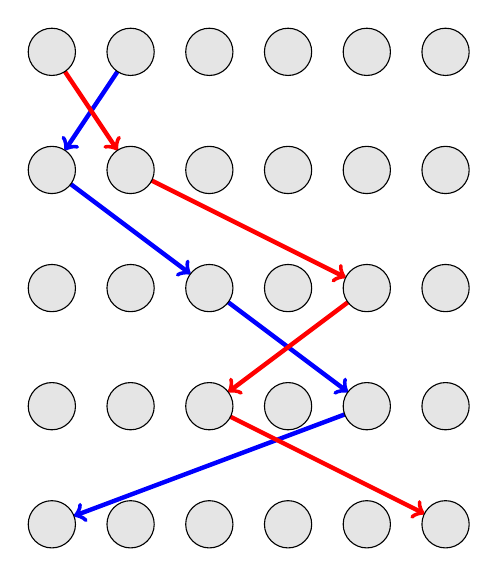
\begin{tikzpicture}

% Draw the arrows for the bad path
\draw[color=blue,ultra thick,->] (.834,-.250) -- (.166,-1.250);
\draw[color=blue,ultra thick,->] (.24,-1.68) -- (1.76,-2.82);
\draw[color=blue,ultra thick,->] (2.24,-3.18) -- (3.76,-4.32);
\draw[color=blue,ultra thick,->] (3.719,-4.605) -- (.281,-5.894);

% Draw the arrows for the good path
\draw[color=red,ultra thick,->] (.166,-.250) -- (.834,-1.250);
\draw[color=red,ultra thick,->] (1.268,-1.634) -- (3.732,-2.866);
\draw[color=red,ultra thick,->] (3.76,-3.18) -- (2.24,-4.32);
\draw[color=red,ultra thick,->] (2.268,-4.634) -- (4.732,-5.866);

% Draw all the rows and columns
\foreach \x in {0,1,...,5} \foreach \y in {0,-1.5,...,-6} {
    \filldraw[draw=black,fill=lightgray!40] (\x,\y) circle (.3);
}

\end{tikzpicture}
\end{document}
